\chapter{Experiments}\label{chapter:experiment}

\section{Case studies}
\paragraph{Dijkstra’s algorithm for mutual exclusion}
\paragraph{Dijkstra’s algorithm for mutual exclusion with a token}
\paragraph{Other mutual exclusion algorithms}
\paragraph{Dining philosophers}
\paragraph{Cache coherence protocols}
\paragraph{Termination detection}
\paragraph{Dining cryptographers}
\paragraph{Leader election}
\paragraph{Token passing}

\section{Dodo}
Dodo supports there interpretations (trap, siphon and flow).
Run for every system with  4 algorithms (L*, NL*, KV, RS). 
After that, it plotted the graphs to compare the learned time 
of theses algorithms.

For easier analysing, we use the library mathplot for 
plotting our graph.

\section{Results}
They represent the result of token-passing learning precess.
The color blue means that we can learn while the red one 
indicates the cases that we can not learn.
In the plotted graph we can compare the learning time of for 
algorithm.

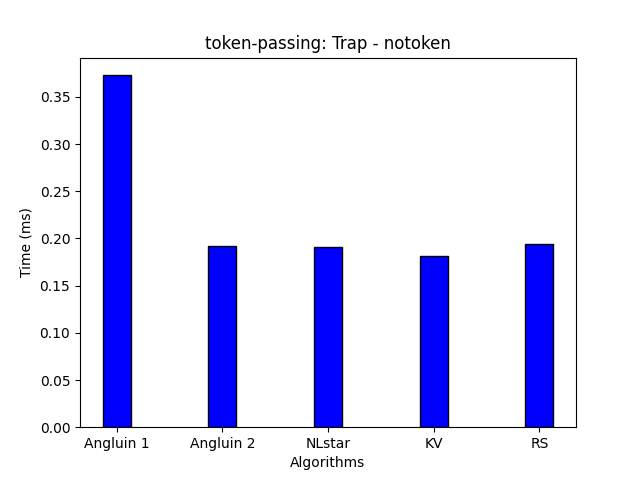
\includegraphics[scale=0.5]{figures/Trap_notoken.png}
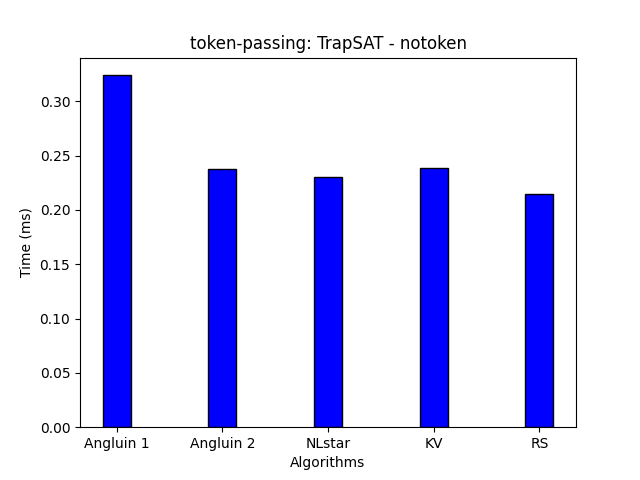
\includegraphics[scale=0.5]{figures/TrapSAT_notoken.png}

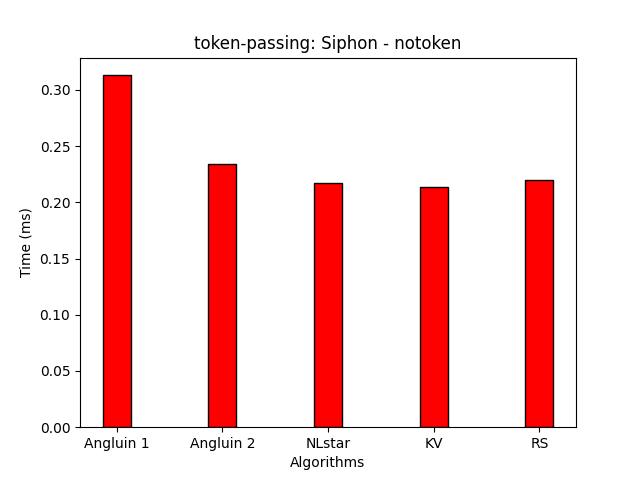
\includegraphics[scale=0.5]{figures/Siphon_notoken.png}
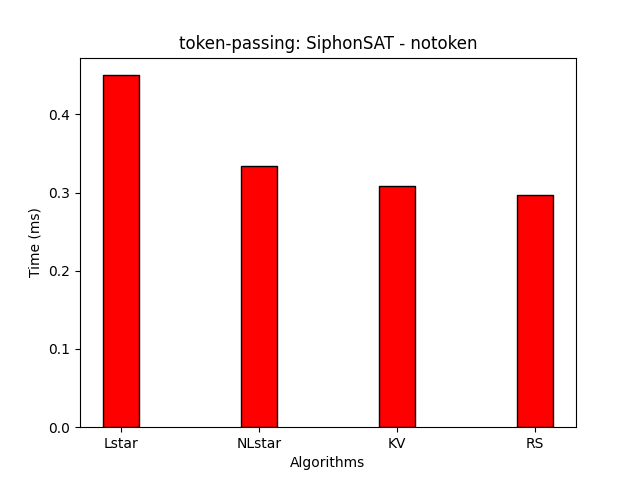
\includegraphics[scale=0.5]{figures/SiphonSAT_notoken.png}


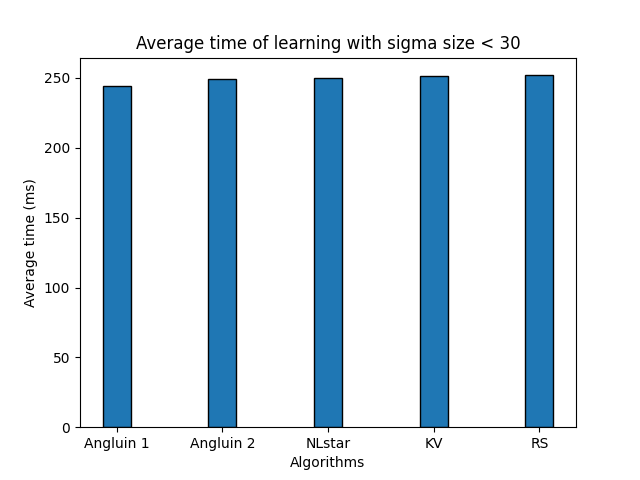
\includegraphics[scale=0.75]{figures/average_time2.png}

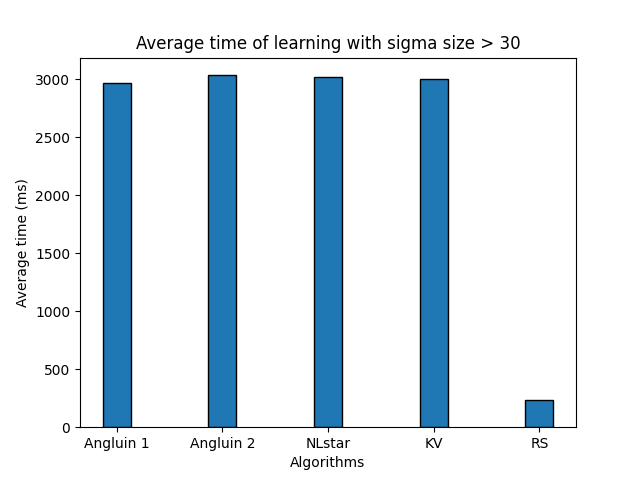
\includegraphics[scale=0.75]{figures/average_time3.png}



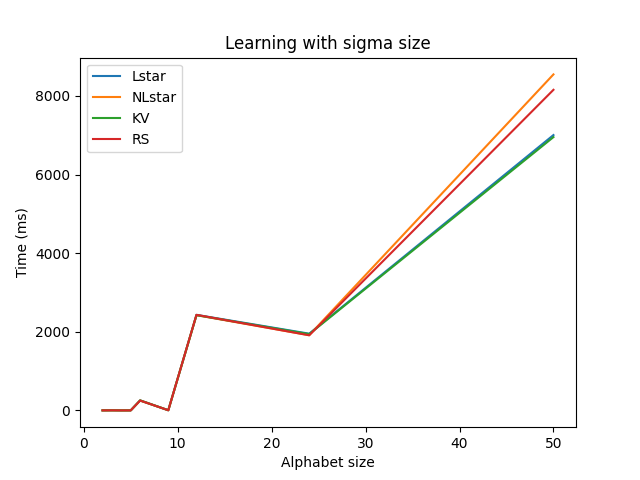
\includegraphics[scale=0.75]{figures/sigma_size.png}

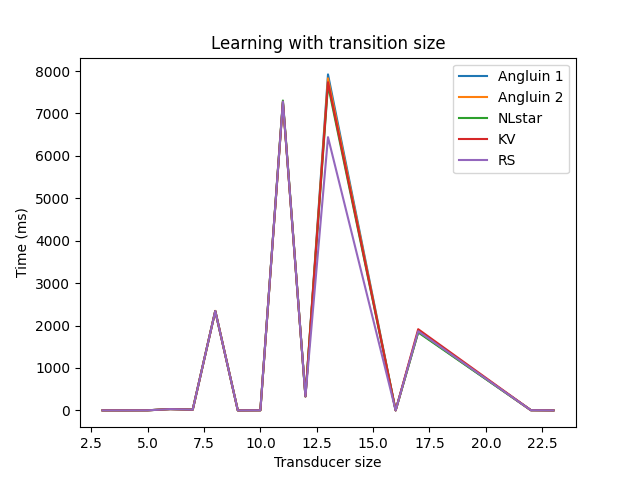
\includegraphics[scale=0.75]{figures/transition_size.png}

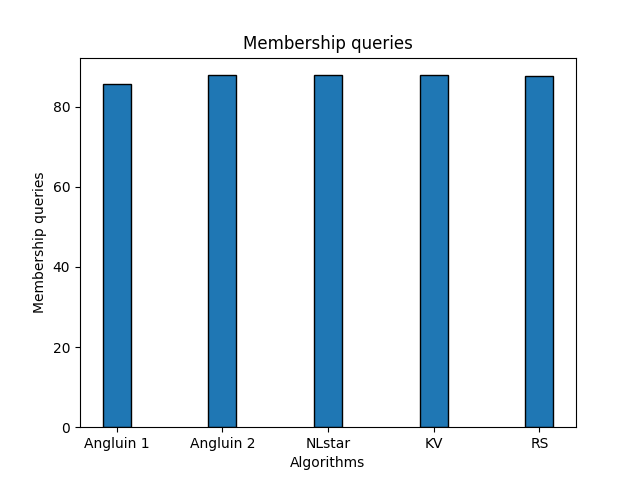
\includegraphics[scale=0.75]{figures/average_membership.png}

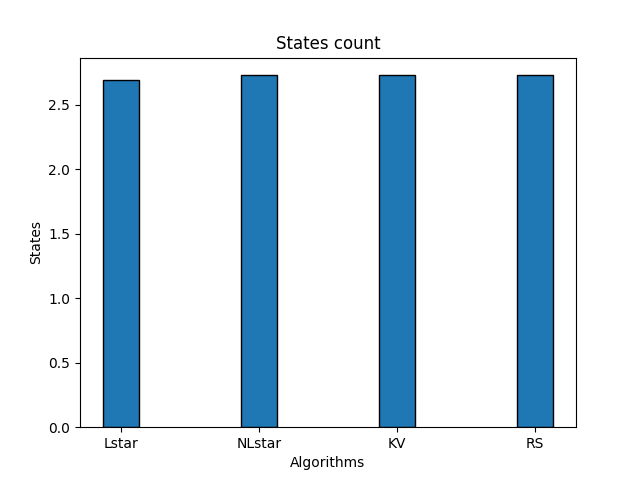
\includegraphics[scale=0.75]{figures/average_stateCount.png}